% !TEX root = ../main.tex
\newpage
\section{The Theta Neuron Model} \label{TheThetaNeuronModel}
A number of neuron model families have been identified, and often there exists a continuous change of variables from models of the same family into a \textit{canonical} model that can represent the whole family \cite{Hoppensteadt2001CanonicalNM}. As the transformation is not required to be invertible, we can study the universal neurocomputational properties of the family in a low dimensional model.
It was Hodgkin \cite{Hodgkin1948} who classified neurons into two types based on their excitability, upon experimenting with the electrical stimulation of cells. Class 1 models begin to spike at an arbitrarily slow rate, and the spiking frequency increases when the applied current is increased. Class 2 models spike as soon as their internal threshold is exceeded and the spiking frequency stays relatively constant within a certain frequency band \cite{Hoppensteadt2001CanonicalNM}.

\subsection{Model description} \label{sec:TheThetaNeuronModelDescription}
In \cite{Ermentrout1986}, a class 1 canonical phase model was proposed:
\begin{align}
\dot{\theta} = (1-\cos \theta)+(1+\cos \theta) \cdot I \qquad \theta \in \T \label{eq:thetaneuron}
\end{align}
with $I$ a bifurcation parameter on the supplied current. We can visualise the dynamics on the unit circle, like in Figure \ref{fig:thetaneuronbifurcationtikz}. The neuron produces a spike when $\theta$ surpasses $\pi$, upon which $\theta \leftarrow -\pi$. 

\begin{figure}[H]
\minipage{0.33\linewidth}
\centering
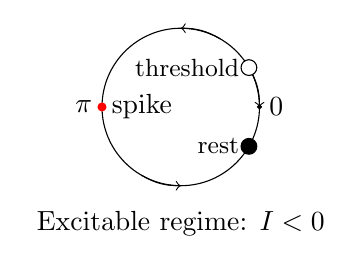
\begin{tikzpicture}
    \draw (0,0) circle [radius=1];
    \draw (0,-1.2) node[below]{Excitable regime: $I < 0$};
    \draw (-1,0) node[left]{$\pi$};
    \draw[fill=black, black] (1,0) circle [radius=0.025];
    \draw (1,0) node[right]{0};
    \draw[fill=red, red] (-1,0) circle [radius=0.05];
    \draw (-1,0) node[right]{spike};
    
    \draw[black, ->] (0.866, 0.5)to[out=-60,in=90](1,0);
    \draw[fill=white, draw=black] (0.866,0.5) circle [radius=0.1];
    \draw (0.866,0.5) node[left]{\small{threshold}};
    
    \draw[fill=black, draw=black] (0.866,-0.5) circle [radius=0.1];
    \draw (0.866,-0.5) node[left]{\small{rest}};
    
    \draw[black, ->] (0.5,0.866)to[out=150,in=0](0,1);
    \draw[black, ->] (-0.5,-0.866)to[out=-30,in=180](0,-1);
\end{tikzpicture}
\endminipage
\minipage{0.33\linewidth}
\centering
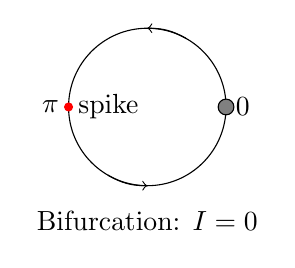
\begin{tikzpicture}
    \draw (0,0) circle [radius=1];
    \draw (0,-1.2) node[below]{Bifurcation: $I = 0$};
    \draw (1,0) node[right]{0};
    \draw[fill=red, red] (-1,0) circle [radius=0.05];
    \draw (-1,0) node[right]{spike};
    \draw (-1,0) node[left]{$\pi$};
    
    \draw[fill=gray, draw=black] (1,0) circle [radius=0.1];
    
    \draw[black, ->] (0.5,0.866)to[out=150,in=0](0,1);
    \draw[black, ->] (-0.5,-0.866)to[out=-30,in=180](0,-1);
\end{tikzpicture}
\endminipage
\minipage{0.33\linewidth}
\centering
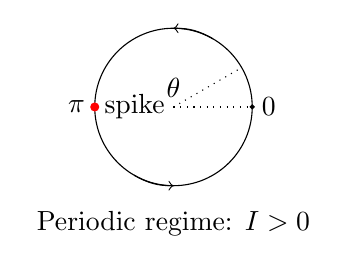
\begin{tikzpicture}
    \draw (0,0) circle [radius=1];
    \draw (0,-1.2) node[below]{Periodic regime: $I > 0$};
    \draw (-1,0) node[left]{$\pi$};
    \draw (1,0) node[right]{0};
    \draw[fill=black, black] (1,0) circle [radius=0.025];
    \draw[fill=red, red] (-1,0) circle [radius=0.05];
    \draw (-1,0) node[right]{spike};
    
    \draw[black, dotted] (0,0)to(1,0);
    \draw(0,0) node[above]{$\theta$};
    \draw[black, dotted] (0,0)to(0.866,0.5);
    
    \draw[black, ->] (0.5,0.866)to[out=150,in=0](0,1);
    \draw[black, ->] (-0.5,-0.866)to[out=-30,in=180](0,-1);
\end{tikzpicture}
\endminipage
\caption{SNIC bifurcation of the theta neuron model. A spike occurs when $\theta = \pi$. For $I < 0$, the neuron is in a rest state but \textsl{excitable}. For $I > 0$, $\dot{\theta} > 0$ so that $\theta$ moves continuously around the circle and we can observe \textsl{periodic} sustained spiking. The saddle-node bifurcation occurs at $I = 0$, so that $\theta$ will spike when it is larger than 0.}
\label{fig:thetaneuronbifurcationtikz}
\end{figure}

We can recognise the features of the class 1 model in Figure \ref{fig:ThetaNeuronResponseToCurrent}. This makes \eqref{eq:thetaneuron} the normal form of the \textit{saddle-node-on-invariant-circle} ($\SNIC$) bifurcation \cite{Luke2013}.

\begin{figure}[H]
\centering
\includegraphics[width = \textwidth]{../Figures/ThetaNeuronResponseToCurrent.pdf}
\caption{Properties of the theta neuron model, with solutions of \eqref{eq:thetaneuron} in blue, spikes marked in dotted lines, and the current $I$ in red. Left: the spike frequency of $\theta$ increases as $I$ is increased over time, which is the distinguishing feature of class 1 canonical models. Middle: spikes occur within a finite time period when $I > 0$ and within infite time when $I = 0$. Right: when $I$ is large, the neuron \textsl{bursts}.}
\label{fig:ThetaNeuronResponseToCurrent}
\end{figure}

Equilibria only exist for the \textsl{excitable} regime $I < 0$: 
\begin{align*}
\dot{\theta} &= 1-\cos \theta+I+I \cdot \cos \theta = (I+1)+(I-1) \cdot \cos \theta \\
\theta^{\ast}_{1, 2} &= \pm \arccos \left(\frac{I+1}{1-I}\right)+2 \pi n
\end{align*}
We can find the stability of the equilibria through:
\begin{align*}
\frac{\mathop{d}}{\mathop{d \theta}}((1-\cos \theta)+(1+\cos \theta) \cdot I) &= \sin \theta-\sin \theta \cdot I = (1-I) \cdot \sin \theta
\end{align*}
In the equilibria this yields:
\begin{align*}
\frac{\mathop{d}}{\mathop{d \theta}}\left( \theta^{\ast}_{1, 2} \right) &= \pm(1-I) \cdot \sqrt{1-\frac{I+1}{1-I}}=\pm(1-I) \cdot \frac{2 \sqrt{-I}}{1-I} = \pm2 \sqrt{-I}
\end{align*}
This yields a stable equilibrium point for $\theta^{\ast}_{1}$ and an unstable for $\theta^{\ast}_{2}$. This means that as $\theta$ gets perturbed above $\theta^{\ast}_{2}$, a spike occurs and $\theta$ converges to $\theta^{\ast}_{1}$. This is demonstrated in Figure \ref{fig:ThetaModelEquilibriumPoints}.
\begin{figure}[H]
\centering
\includegraphics[width = \textwidth]{../Figures/ThetaModelEquilibriumPoints.pdf}
\caption{Equilibria $\theta^{\ast}$ for different values of $I$. Left: $I = -1$ yields $\theta^{\ast}_{1,2} = \pm \frac{\pi}{2}$, one of the simulations is started exactly on the unstable equilibrium. Middle: $I = -0.5$. Right: bifurcation diagram of the \SNIC bifurcation, with the stable equilibria in blue, and the unstable in red.}
\label{fig:ThetaModelEquilibriumPoints}
\end{figure}


\subsection{Solutions for static currents} \label{sec:TheThetaNeuronModelSolutionPeriodics}
Gaining insight into \eqref{eq:thetaneuron} is hard, due to the difficulty of finding an analytical solution. However, it has been noted that there exists a simple transformation which yields (see \ref{app:TransformationToQIF}):
\begin{align}
V &\equiv \tan \left( \frac{\theta}{2} \right) \label{eq:QIFtransformation} \\
\dot{V} &= V^2 + I \label{eq:QIFmodel}
\end{align}
This model is called the \textsl{Quadratic Integrate and Fire model} (\QIF). \eqref{eq:QIFmodel} models the membrane potential of a neuron, which spikes to $=\infty$ when the neuron spikes and is reset at $-\infty$. The transformation \eqref{eq:QIFtransformation} is continuous between spikes, so insights from a solution for $V$ can be transformed directly. The equilibria of the \QIF model are simply $\pm \sqrt{I}$ so that we can express $\theta^{\ast}_{1, 2} = 2 \cdot\arctan \left( \mp \sqrt{I} \right)$ \cite{Gutkin2014}. \\

The solution for the excitable regime $I < 0$ is :
\begin{align}
V(t) = \frac{2 \sqrt{-I}}{1 - e^{2 t \sqrt{-I}}}-\sqrt{-I} \label{eq:ThetaNeuronModelSolutionPeriodicExcitable}
\end{align}
The solution at the bifurcation $I = 0$ is :
\begin{align}
V(t) = \frac{-1}{t} \label{eq:ThetaNeuronModelSolutionPeriodicBifurcation}
\end{align}
The solution for the periodic regime $I > 0$ is :
\begin{align}
V(t) = -\sqrt{I} \cdot \cot (t \sqrt{I}) \label{eq:ThetaNeuronModelSolutionPeriodic}
\end{align}
The solutions to \eqref{eq:ThetaNeuronModelSolutionPeriodicExcitable}-\eqref{eq:ThetaNeuronModelSolutionPeriodic} are described in \ref{app:ThetaModelSolutions}. Solutions for $\theta$ are found by taking the inverse of the transformation \eqref{eq:QIFtransformation}.

\subsection{Frequency response} \label{sec:TheThetaNeuronModelFrequencyResponse}
As we already saw in Figure \ref{fig:ThetaNeuronResponseToCurrent}, an increasing current increases the spiking frequency. We can compute this relationship by measuring how long it takes for $V$ to reach a spike: we solve \eqref{eq:ThetaNeuronModelSolutionPeriodic} for $t$ at $V(t) = +\infty$ in \ref{app:ThetaModelFrequencyResponse}. This yields the oscillation period $T = \frac{\pi}{\sqrt{I}}$ which we can see in Figure \ref{fig:ThetaNeuronResponseToCurrentPeriod}. 

We know that when $\theta > \theta^{\ast}_{2}$ a spike occurs. But the time that it takes to reach the spike can be arbitrarily long, depending on how far we are over $\theta^{\ast}_{2}$. So, spikes will occur, but after a delay that is dependant on the stimulus. Explicitly, if we perturb $\theta(0) = \theta^{\ast}_{2} + \varepsilon$ we obtain from  \cite{Gutkin2014}:
\begin{align*}
T_{\text {spike}} = \frac{-\tanh ^{-1}\left(1+\frac{\epsilon}{\sqrt{I}}\right)}{\sqrt{I}}
\end{align*}
The delay to the spike blows up as $\varepsilon \rightarrow$ 0 so that spikes may occur after a very large delay.

\begin{figure}[H]
\centering
\includegraphics[width = 0.75\textwidth]{../Figures/ThetaNeuronResponseToCurrentPeriod.pdf}
\caption{Frequency response of the theta model, with theoretical results in blue, and experimental results in black dots. For $I \leq 0$ the spike period is infinite, which is why we see the solutions to \eqref{eq:thetaneuron} approach $\theta = 0$ for $I = 0$.}
\label{fig:ThetaNeuronResponseToCurrentPeriod}
\end{figure}

In most of our future work, $I$ will not be a static current. We ask ourselves: how sensitively does $T$ depend on $I$ when $I$ is perturbed? We can measure this as a \textsl{relative} perturbation using $\mathop{dI}/I$ and $\mathop{dT/T}$ \cite{IntroductionModelingDynamics} :
\begin{align*}
\left| \frac{dT}{dI} \frac{I}{T} \right| &= \left| \frac{dT / T}{dI / I}\right| 
= \left|- \frac{\pi}{2} \left(\frac{1}{\sqrt{I}}\right)^3 \frac{I}{T} \right| 
= \left| \frac{\pi}{2} \left(\frac{T}{\pi}\right)^3 \frac{I}{T} \right| 
= \frac{1}{2} \left|\left(\frac{T}{\pi}\right)^2 \cdot \left(\frac{\pi}{T}\right)^2 \right| = \frac{1}{2}
\end{align*}
Hence, a 1\% change in $I$ will result in a 0.5 \% change in the period.


\subsection{Phase response} \label{sec:TheThetaNeuronModelPhaseResponse}
Perturbations on the period can also be understood from the perspective of the phase. Changes to the phase $\theta$ can delay or advance the event of a spike, and in general this depends on exactly when the stimulus occurs. The phase response curve (\PRC) gives us exactly that relation \cite{Perez2020, Gutkin2014}.

For infinitesimally small perturbations to the phase, we can find the \PRC as the \textsl{adjoint} of the solution as:
\begin{align*}
\PRC(t)=\frac{1}{d V / d t}=\frac{1}{2 \sqrt{I}}(1-\cos (2 \cdot t \cdot \sqrt{I}))
\end{align*}


\subsection{Networks of theta neurons}
We can easily extend the model to networks of neurons:
\begin{align}
\dot{\theta}_{i} &=\left(1-\cos \theta_{i}\right)+\left(1+\cos \theta_{i}\right) \cdot \left[\eta_{i} + \kappa \cdot I_{i}(t)\right] \qquad \theta_i \in \T^N  \label{eq:thetaneuronnetwork} \\
I_{i}(t) &=\frac{1}{\kmean} \sum_{j=1}^{N} A_{i j} \cdot \mathcal{P}_{n}(\theta_{j}) \label{eq:thetaneuronnetworkcurrent}
\end{align}
where the excitability $\eta_i$ is drawn from a distribution $g(\eta \rvert \eta_0, \sigma)$ and $\mathcal{P}(\theta)  = a_n(1 - \cos \theta)^n$ models synaptic coupling by a pulse-shaped signal, emitted when a neuron fires. $n$ models the sharpness of the pulse, and $a_n$ is a normalisation constant. We will take $n=2$ from here in as in\cite{Luke2013}, \cite{OttAntonsen2017}, \cite{Martens2020}. 


Another type of coupling is proportional to the difference in voltage between neurons \cite{Martens2020}. Note that for a fully connected network, \eqref{eq:thetaneuronnetworkcurrent} reduces to the scenarios in \cite{Luke2013} and \cite{Martens2020}.

In \eqref{eq:thetaneuronnetwork} we see everything come together: changes to the phase $\theta_i$ come from $\dtheta_i$, which in turn depends on $I$, which depends on all phases in the network.



